\documentclass{article}

\usepackage[utf8]{inputenc}
\usepackage[margin=2cm]{geometry}
\usepackage{amsfonts,amsmath,amssymb}
\usepackage[T1]{fontenc}
\usepackage[french]{babel}
\usepackage{array}
\usepackage{url}
\usepackage{graphicx}
\usepackage{tikz}
\usetikzlibrary{arrows,automata,shapes}
\usepackage[nottoc,notlot,notlof]{tocbibind}
\usepackage{caption}
\usepackage{minted}
\usepackage{fancybox}
\usepackage{fancyhdr}
\usepackage{hyperref}
\usepackage{pgfgantt}

\pagestyle{fancy}
\fancyhead{}
\fancyfoot{}
\fancyhead[L]{\slshape \MakeUppercase{Hex Project}}
%\fancyhead[R]{\slshape Ismail ELOMARI ALAOUI - Nicolas LE QUEC - Vincent RIDACKER - Alexandre GISSAUD }
\fancyfoot[C]{\thepage}
\fancyfoot[R]{\slshape Encadré par: Guillaume Mercier }
\fancyfoot[L]{\slshape I1-P6-Groupe 2}
\renewcommand{\footrulewidth}{1pt}
\parindent 0ex
\renewcommand{\baselinestretch}{1,5}
\newcommand{\tikzlogo}{Ti\emph{k}Z}
\usepackage{color}
\usepackage{listings}
\definecolor{darkWhite}{rgb}{0.94,0.94,0.94}
 
\lstset{
  aboveskip=3mm,
  belowskip=-2mm,
  backgroundcolor=\color{darkWhite},
  basicstyle=\footnotesize,
  breakatwhitespace=false,
  breaklines=true,
  captionpos=b,
  commentstyle=\color{red},
  deletekeywords={...},
  escapeinside={\%*}{*)},
  extendedchars=true,
  framexleftmargin=16pt,
  framextopmargin=3pt,
  framexbottommargin=6pt,
  frame=tb,
  keepspaces=true,
  keywordstyle=\color{blue},
  language=C,
  literate=
  {²}{{\textsuperscript{2}}}1
  {⁴}{{\textsuperscript{4}}}1
  {⁶}{{\textsuperscript{6}}}1
  {⁸}{{\textsuperscript{8}}}1
  {€}{{\euro{}}}1
  {é}{{\'e}}1
  {è}{{\`{e}}}1
  {ê}{{\^{e}}}1
  {ë}{{\¨{e}}}1
  {É}{{\'{E}}}1
  {Ê}{{\^{E}}}1
  {û}{{\^{u}}}1
  {ù}{{\`{u}}}1
  {â}{{\^{a}}}1
  {à}{{\`{a}}}1
  {á}{{\'{a}}}1
  {ã}{{\~{a}}}1
  {Á}{{\'{A}}}1
  {Â}{{\^{A}}}1
  {Ã}{{\~{A}}}1
  {ç}{{\c{c}}}1
  {Ç}{{\c{C}}}1
  {õ}{{\~{o}}}1
  {ó}{{\'{o}}}1
  {ô}{{\^{o}}}1
  {Õ}{{\~{O}}}1
  {Ó}{{\'{O}}}1
  {Ô}{{\^{O}}}1
  {î}{{\^{i}}}1
  {Î}{{\^{I}}}1
  {í}{{\'{i}}}1
  {Í}{{\~{Í}}}1,
  morekeywords={*,...},
  numbers=left,
  numbersep=10pt,
  numberstyle=\tiny\color{black},
  rulecolor=\color{black},
  showspaces=false,
  showstringspaces=false,
  showtabs=false,
  stepnumber=1,
  stringstyle=\color{gray},
  tabsize=4,
  title=\lstname,
}

\begin{document}


\begin {titlepage}
  \begin{center}
      \vspace*{1cm}
    \Large{\textbf{Hex Project}}\\
    \Large{\textbf{Rapport de projet}}
    \vfill
    \begin{figure}[h]
        \centering
        \includegraphics[scale=0.5]{MATMECA.PNG}
    \end{figure}
    \vfill    
    
    %\line{1,0}{400}\\[1mm]
    \huge{\textbf{Projet de programmation - S6}}\\[3mm]
    \Large{\textbf{-- I1 - ENSEIRB-MATMECA --}}\\[1mm]
    \Large{\textbf{Encadrants: M. David RENAULT - M. Guillaume MERCIER }}\\[1mm]    
    %\line{1,0}{400}\\
    \vfill
    Par Ismail ELOMARI ALAOUI - Nicolas LE QUEC - Vincent RIDACKER - Alexandre GISSAUD\\
    \today\\
  \end{center}
\end{titlepage}

 \tableofcontents
%\thispagestyle{empty}
\clearpage
\newpage

\section*{Introduction}
    \subsection*{Contexte}
    Ce rapport a pour objectif de décrire l’ensemble du processus de réalisation d'un projet de programmation en C. Ce projet est conçu par Mr. David RENAULT, le directeur des projets à l'ENSEIRB-MATMECA, pour aider les élèves en première année d’informatique à avoir des compétences basiques voire avancées sur l'utilisation du C. Le projet consiste en l’implémentation d'un jeu appelé HEX, en C.
    Le jeu de $Hex$ est un jeu de société à deux joueurs, qui se joue sur un plateau à cases hexagonales dont les bords sont colorés aux couleurs des joueurs (ici $BLACK$ et $WHITE$), en alternant. Deux joueurs (stratégies) s'affrontent en sélectionnant à chaque tour une case du tableau inoccupée, et en lui assignant sa couleur. Le vainqueur du jeu est celui réussissant à connecter les deux bords de sa couleur par un chemin de cases lui appartenant.\\
    \begin{figure}[h]
        \centering
        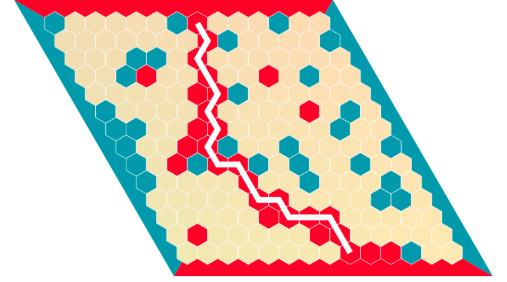
\includegraphics{hexgame.png}
        \caption{Un match de hex}
        \label{fig:hexgame}
    \end{figure}

    \subsection*{Description du sujet}
L'objectif du projet consiste à implémenter un ensemble de fonctions permettant de faire jouer deux joueurs à une partie de Hex. Le code sera décomposé en deux parties distinctes :
\begin{itemize}
    \item Un ensemble de clients implémentant tous une interface commune, gérant leur propre plateau de jeu et jouant chacun selon leur objectif propre. Ces clients sont censés être automatiques : ils doivent décider d'un coup à jouer à l'aide d'un algorithme, sans intervention extérieure.
    \item Un serveur de jeu organisant une partie, faisant jouer chaque client à son tour en lui envoyant les coups joués par son adversaire, enregistrant le coup du client à son tour et notifiant les clients de la fin de la partie.
Le serveur de jeu devra, par l'intermédiaire d'options (décrites dans la section  Détails techniques) permettre de sélectionner la forme du plateau (avec des graphes de tailles et de formes différentes).
\end{itemize}

 Plusieurs problématiques se mettent en valeur de façon assez intuitive:
 \begin{itemize}
    \item Une partie se termine-t-elle forcément? 
    \item Comment un serveur peut-il être proprement codé?
    \item Comment le serveur implémenté peut-il assurer la sécurité et la transparence du jeu? 
    \item Comment un joueur peut-il être représenté?
    \item Vu que M. David RENAULT a créé une ligue de jeu, les joueurs doivent être représentés par des librairies dynamiques afin de faciliter l'organisation du jeu par le serveur du jeu. Comment peut-on assurer la bonne compilation de n'importe quel joueur, la stabilité et la robustesse de notre serveur de jeu?
    \end{itemize}
  Ce sont de façon relativement succincte, les consignes principales à résoudre et à respecter pendant notre projet.
\newpage
 


 \section{Méthode de travail}
    \subsection{Répartition des tâches}
    Tout d'abord, notons que ce projet a été du début à la fin un travail d'équipe complet, dans lequel nous avons appris tout du long à beaucoup échanger et à travailler ensemble, tout en se répartissant les tâches quand cela était nécessaire. Nous pensons que tout ce qui peut fracasser une équipe de programmeurs est la mal-structuration du projet. Nous pensons avoir fait de notre mieux pour éviter cette catastrophe.
    
    L'organisation du travail a été cependant très simple. \`A chaque séance, nous travaillions en vocal (généralement sur Discord). Le travail a été réparti sur la base du volontariat et de la bonne volonté. Aucun document décrivant les responsabilités et tâches d'un membre n'a été rédigé. \`A la place, le découpage de la charge de travail a été décidé oralement et chaque membre a été libre de choisir ce dont il souhaitait s'occuper.
    
    La totalité des tâches à réaliser n'a pas été définie avant leur réalisation. Le projet s'est construit de manière incrémentale. Bien qu'il a quand même fallu une vision d'ensemble et décider d'une direction quant à la structuration du projet. Les tâches ont donc plutôt été décidées en même temps que l'avancement du projet. Lorsqu'un membre a terminé une tâche, il en décide d'une autre à réaliser et discute avec les autres membres de sa validité et de sa pertinence dans le projet. Une fois validée, la tâche est alors attribuée à quelqu'un et ainsi de suite.
    
    Cette organisation est très légère en terme de mise en place. Il n'y a eu aucun réel contrôle de travail. Ce genre d'organisation n'est probablement possible que dans un petit groupe et est vulnérable aux comportements égoïstes. Cette méthode de travail est basée sur la confiance et la bonne volonté de chaque membre. Elle a été cependant plutôt bénéfique pour notre groupe qui s'est très bien entendu dès le début ce qui a permis une atmosphère de travail plus agréable. Elle a également permis une certaine réactivité face aux problèmes. Lorsqu'un membre avait besoin d'aide, n'importe quel autre membre pouvait se joindre à lui puisque aucune tâche n'était individuellement attribuée et délimitée dans le temps précisément.
    
    \subsection{Thor Project}
    Nous avons utilisé la Forge (le serveur $Thor Project$) de l'ENSEIRB-MATMECA pour gérer les différentes versions de notre projet. L'évolution du projet visible sur cette Forge peut mettre en évidence nos progrès en tant que programmeurs, de niveau modeste, en C.\\
    Nous avons utilisé comme il nous l'avait été demandé LaTeX pour rédiger ce rapport. Afin de simplifier le travail simultané sur l'écriture de ce rapport, nous avons utiliser $Overleaf$, un éditeur LaTeX en ligne.\\

    \subsection{\textit{Makefile}}
Nous avons utilisé l'outil d'aide à la compilation \textbf{$make$}, en réalisant un \textbf{$Makefile$}.
Ce fichier fournit plusieurs régles :
\begin{itemize}
    \item Une règle $build$ qui compilera l'ensemble du code,
    \item Une règle $test$ qui compilera les tests, sans les exécuter.
    \item Une règle $install$ qui copiera les exécutables (un exécutable nommé $server$, un exécutable $alltests$, et un nombre non spécifié de fichiers $.so$) à l'intérieur du répertoire désigné.
    \item Une règle $clean$ qui supprimera les fichiers compilés et installés.
\end{itemize}

    \subsection{Architecture du répertoire \textit{GIT}}
    Notre dépôt contient plusieurs répertoires: $src$ qui contient tous les codes sources utilisés pour passer les tests, créer un serveur de jeu robuste et des stratégies plus ou moins fiables.
    Ensuite, le répertoire $test$ contient plusieurs fichiers utilisés pour assurer le bon fonctionnement de nos codes sources. Enfin, le répertoire $"report"$ contient ce rapport en version \LaTeX (code source).

\newpage

\section{Preuve de terminaison}
De manière assez intuitive, il est possible de se rendre compte qu'une partie de Hex se termine forcément avec un unique vainqueur. Il s'agit néanmoins d'un résultat non trivial dont la preuve est liée au théorème de Brouwer et accessible dans document suivant de D. Gale:
\url{http://www.math.pitt.edu/~gartside/hex_Browuer.pdf}
\\
Bref, comment peut-on savoir qu'un joueur gagnera sur une partie de format hexagonal?\\
Supposons que chaque hexagonal est plein.\\
\begin{figure}[ht]
    \centering
    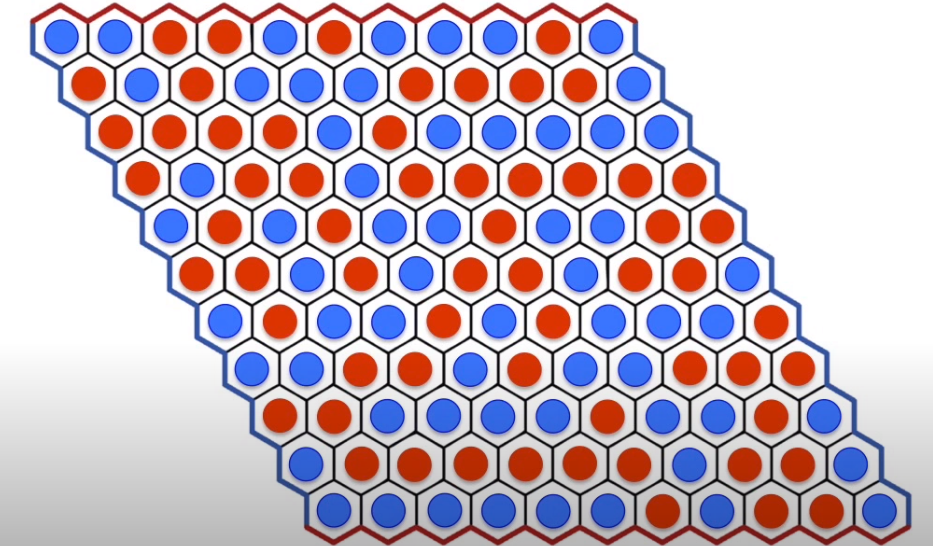
\includegraphics[scale=0.5]{hexplein.png}
    \label{fig:hexplein}
\end{figure}
\\
Ensuite, on dessine en noir chaque arête qui sépare un hexagonal bleu d'une autre rouge, ou qui sépare un hexagonal d'une couleur à une bordure d'une autre couleur.\\
\begin{figure}[ht]
    \centering
    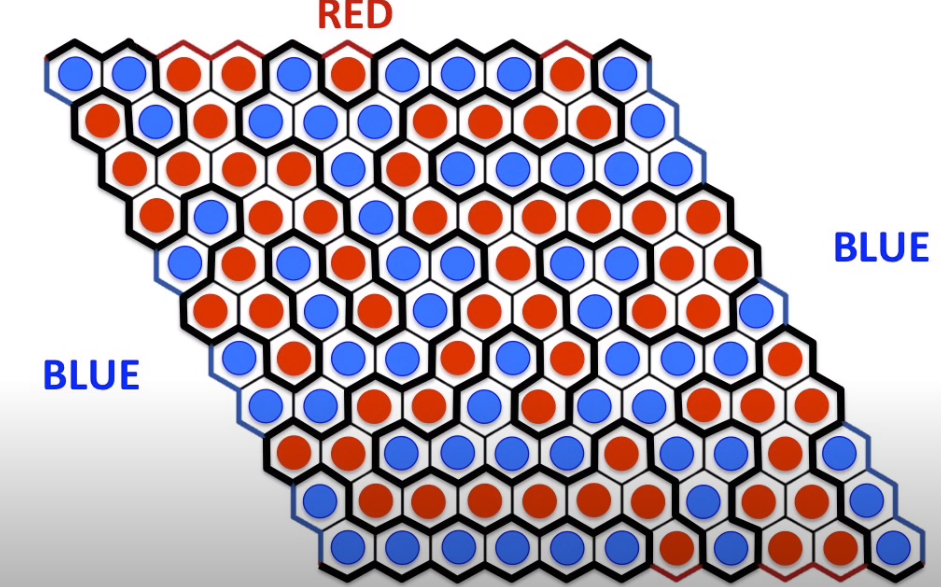
\includegraphics[scale=0.5]{chaines.png}
    \label{fig:chaines}
\end{figure}
\\
Nous remarquons qu'il y a exactement deux chaînes noirs dessinées. Chaque chaîne séparant le bleu du rouge, est connectée du bout supérieur (soit droit soit gauche) au bout inférieur. C'est pourquoi il y a toujours un chemin gagnant.\\
\begin{figure}[ht]
    \centering
    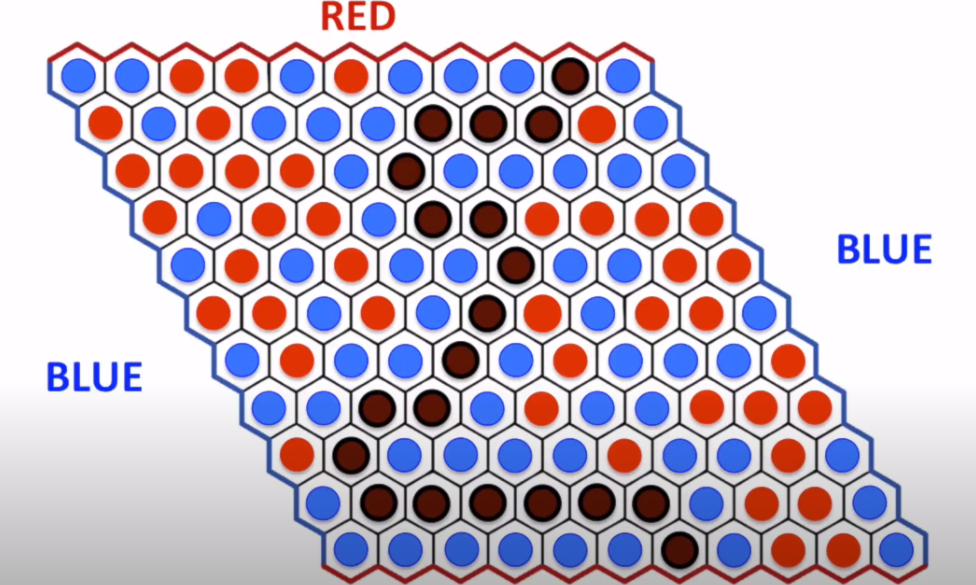
\includegraphics[scale=0.5]{chemingagne.png}
    \label{fig:chemingagne}
\end{figure}
\\
Il suffit donc de prouver l'existence de ces deux fameuses chaînes dans n'importe quel plateau de jeu. Mais, comment peut-on aborder cette preuve?\\
Nous devons d'abord comprendre la magie de la jonction d'hexagones qui se rencontrent: Pour chaque jonction, il y a 2 ou 0 arêtes noires de ces chaînes, même dans les bouts du plateau de jeu.\\
\begin{figure}[ht]
    \centering
    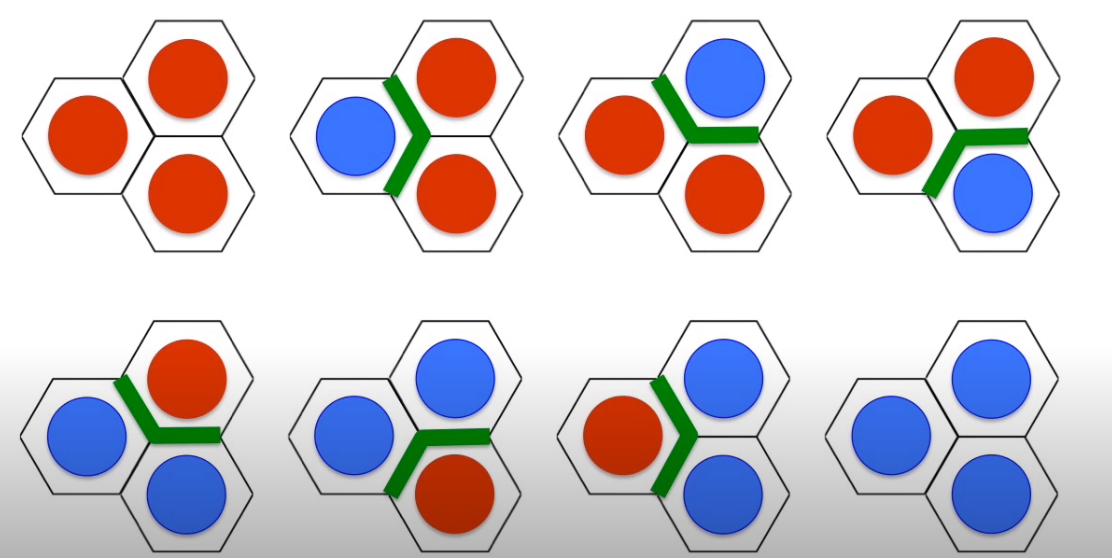
\includegraphics[scale=0.5]{joint.png}
    %\label{fig:chemingagne}
\end{figure}
\\
\begin{figure}[ht]
    \centering
    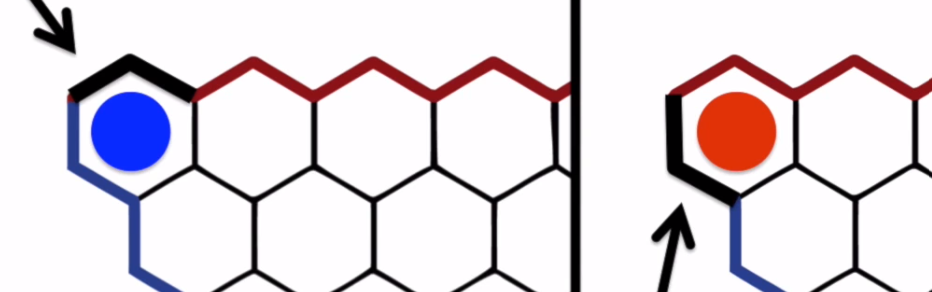
\includegraphics[scale=0.5]{cornerjoint.png}
    %\label{fig:chemingagne}
\end{figure}
\\
Et comme, dans ces jonctions le nombre d'arêtes noires est soit 0 soit 2, la chaîne continue de grandir, car sinon il existerait une jonction avec une seule arête noire. Mais, continue-t-elle de grandir infiniment?\\
La chaîne ne peut pas se reconnecter à elle-même car on aurait une jonction illégale à trois arêtes noirs. La seule autre option est que la chaîne commence d'un bout supérieur (gauche ou droit) et se termine sur le bout inférieur (gauche ou droit) respectivement. Et voilà nos deux fameuses chaînes ont été créées. Sur ce, notre preuve est complète.\\
Pourtant, cet argument ne marche pas pour les plateaux de jeux carrés. Et voici un élégant (certes mais aussi trivial) contre-exemple.\\
\begin{figure}[h]
    \centering
    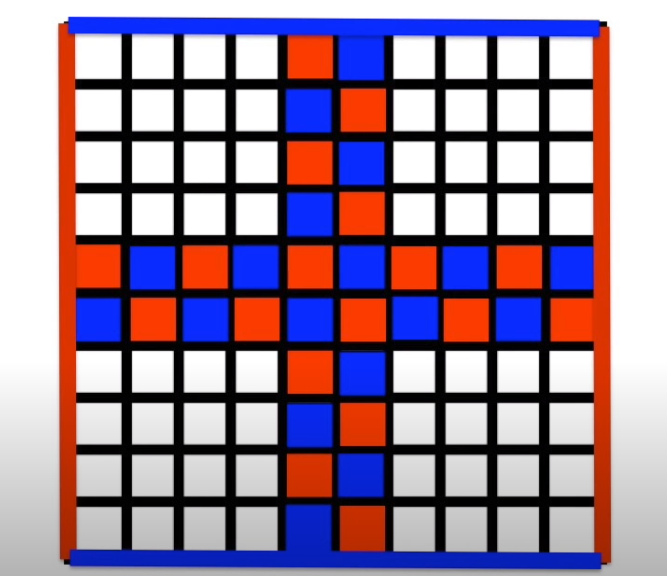
\includegraphics[scale=0.5]{squaregrid.png}
    %\label{fig:chemingagne}
\end{figure}

\section{Structuration du projet}
Maintenant que nous avons prouvé la terminaison pour un plateau du jeu hexagonal. Nous nous concentrerons sur ce type de plateau pour la majorité de notre projet tout en implémentant comme il nous est demandé les autres formats (carré et triangulaire).\\
On passe ainsi à la structuration du projet, cette section décrit les types de données servant de briques de base à la réalisation du sujet. Pour la suite, on supposera que les deux joueurs sont représentés par les entiers 0 ($BLACK$) et 1 ($WHITE$). Le joueur $BLACK$ est celui débutant la partie. Les définitions des coups et des graphes utilisés sont déclarés et définis dans $move.h$  et $graph.h$.
\subsection{\textit{strut graph\_t}}
 Les composants du graphe sont des matrices creuses définies par la $GNU$ $Scientific$ $Library$. Le graphe contient:
 \begin{itemize}
     \item Un nombre de sommets $num\_vertices$ (ou n pour simplifier). 
     \item La matrice $t$ est une matrice d'adjacence de taille n*n représentant les arêtes du graphe.
     \item La matrice $o$ est une matrice $2*n$ codant sur chaque ligne les sommets du graphe appartenant au joueur correspondant (donc 0 ou 1). 
 \end{itemize}
 Toute autre fonction en relation avec le plateau du jeu est déclarée sur le fichier $graph\_struct.h$, notamment les fonctions de créations de graphes carrés, hexagonaux et triangulaires. De plus, vous trouverez sur ce fichier des fonctions d'affichage de graphes colorées, de la duplication de graphes et d'autres fonctions d'aide qui \textbf{peuvent} être utilisés plus tard.  Nous vous présentons en titre d'exemple notre fonction qui créer des graphes hexagonaux (cf. figure \ref{fig:graph_hex})


\subsection{\textit{struct move\_t}}
Un coup contient deux champs:
\begin{itemize}
    \item Un indice m tel que $ 0 <= m < num\_vertices$
    \item Une couleur c ($BLACK$ ou $WHITE$), représentant la couleur du joueur qui joue ce coup.
\end{itemize}

\subsection{\textit{struct player}}
Comme l'indique la boucle de jeu fournie par M. David Renault, un joueur contient plusieurs champs sous forme de pointeurs de fonctions qui pointent sur les fonctions implémentant les actions qu'il pourra réaliser lors de son tour de jeu (cf. figure \ref{fig:player}).



\section{Serveur du jeu}
\subsection{Détails techniques}
L'implémentation d'un bon serveur de jeu est basé sur trois consignes, voire contraintes:
\begin{enumerate}
    \item Les différents clients doivent être interopérables entre équipes de projets. \`A cet effet, chaque client est compilé sous la forme d'une bibliothèque partagée (option $-shared$ de $gcc$) et chargeable de manière dynamique, en utilisant les fonctions de la famille $dlopen$, définies dans $dlfcn.h$.
    \item L'interface interdit toute communication dudit plateau entre client et serveur pendant la partie. Ceci nécessite une copie du graphe, initialisée par le serveur, et cette copie aura lieu nécessairement sur le serveur afin d'éviter toute tricherie.
    \item Le serveur devra charger l'ensemble de ses clients de manière dynamique en utilisant la syntaxe suivante :
    \begin{verbatim}
        ./install/server -m [M] -t [T] ./install/player1.so ./install/player2.so
    \end{verbatim}
    Ceci est assurée par l'implémentation d'une fonction $parse\_opts$ qui cherche ces variables $m$ ( qui est la longueur d'un coté du graphe - 1 ) et $t$ (qui est le format du graphe $h$ -hexagonal-, $t$ -triangulaire- ou $c$ -carré-) parmi tous les arguments. Dans le cas o\`u ces variables ne sont pas renseignées, des valeurs par défaut sont utilisées. La bonne lecture des librairies malgré l'ordre des arguments est assurée, comme la contrainte 1 l'indique, par $dlfcn.h$ et la variable globale $optind$, qui est un curseur sur les arguments.  
\end{enumerate}

\subsection{Fonction \textit{is\_winning} / Critère d'arrêt}
 \`A chaque tour, dans la boucle de jeu, le programme doit vérifier si un des joueurs gagne, et alors la partie et arrêtée et on affiche le joueur gagnant. Cette fonctionnalité est implémentée dans la fonction $is\_winning$ qui prend en argument le graphe représentant le plateau ainsi que la forme du plateau.La condition de victoire dans un graphe généralisé consiste à créer un chemin de tuile de sa couleur entre les deux bords de cette même couleur. Pour chercher l'existence d'un tel chemin, nous utilisons un algorithme de parcours en profondeur à partir d'une tuile du bord d'une des couleurs, et en cherchant à atteindre une tuile du bord opposé. Pour implémenter cet algorithme, nous avons eu besoin d'utiliser une pile. Nous avons donc réutiliser le type abstrait de donné implémenter dans un cours précédent.

\subsection{Boucle principale}
Comme indiqué par Mr.Renault sur le pseudo-code de la boucle principale du jeu, notre $main$ commence par:
\begin{itemize}
    \item $Option$ $Parsing$ pour attribuer au variables globales $m$ et $t$ leurs valeurs.
    \item Création d'un tableau de deux $struct$ $player$.
    \item Lecture des librairies dynamiques, à l'aide de $dlopen$ et de notre fonction $make\_player$ (cf. figure \ref{fig:making_of_player}).
    \item Création du graphe représentant le plateau du jeu.
    \item Fabrication d'une copie de ce graphe puis initialisation des graphes des clients.
    \item Proposition d'un coup par le premier client (ce coup sera \textbf{toujours} le premier coup du joueur $BLACK$).
    \item Refus ou acceptation du coup par le deuxième client, puis initialisation des couleurs des deux clients (si le coup est accepté , le premier client est $BLACK$. Sinon, le deuxième hérite cette couleur).
    \item Tant que la condition d'arrêt n'est pas vérifiée, les joueurs jouent l'un après l'autre. Ensuite, la fonction $finalize$ de chaque client est exécutée.
    \item Affichage du graphe après la victoire d'un client.
    \item Fermeture des librairies dynamiques à l'aide de $dlclose$, puis libération de tout ce qui est alloué pendant le jeu par notre fonction $graph\_free$ (cf. figure \ref{fig:free}). 
    
\end{itemize}

\section{Stratégies Implémentées}
Pour respecter l'interopérabilité entre les joueurs, tous nos joueurs respectent l'interface décrite par le fichier \textit{player.h}.
Les stratégies ont été écrites de sortes à être compatibles avec les 3 types de graphes (triangulaire, carré et hexagonal).

Au moins 2 stratégies nous ont été demandées pour valider notre projet, voici donc les stratégies que nous avons implémentés.

\subsection{Joueur hasardeux \textit{Randomista}}
 $Randomista$ (le client créé par le fichier $Randomista.c$) est un client arrogant qui se croit toujours chanceux, donc ne veut pas penser à une stratégie. Il propose le premier coup au hasard, accepte toujours le premier coup de l'adversaire et choisit aléatoirement ses coups parmi les coups possibles.
 \subsection{Joueur d'adjacence \textit{Adjacenta}}
 $Adjacenta$ (le client créé par le fichier $Adjacenta.c$) est un client qui pense avoir résolu les problèmes de la vie moderne. Sa réponse est de ne pas prendre beaucoup temps à chercher une orientation ou un chemin, les gens selon lui réussissent en allant étape par étape, pas à pas. Il propose donc le milieu du graphe ($mid = graph->num\_vertices / 2$ si $m$ est pair, et $mid$ +ou- $m/2$ sinon ) comme premier coup, accepte tous les coups de l'adversaire sauf si ce dernier propose aussi l'indice du milieu du graphe. Après avoir initialisé sa couleur, disons qu'il est $BLACK$ (respectivement $WHITE$), il se dirige donc dans une direction (noté 1) vers le haut (respectivement la droite) en essayant d'augmenter son ordonnée (respectivement son abcisse). Quand il joue, il alterne sa direction (l'autre direction est noté 0) vers le bas (respectivement la gauche) en essayant de minimiser son ordonnée (respectivement son abcisse). S'il ne trouve pas un coup valide sur une direction, il cherche sur l'autre. De plus, il mémorise un coup valide pour le jouer au cas o\`u il ne trouve aucun coup optimisé.\\
 Vu que les algorithmes classiques, en relation avec les graphes ($DIJKSTRA$ par exemple), n'ont pas été utilisés, La complexité de notre algorithme, de proposition des coups $chose\_adjacence$, risque d'être élevée (de l'ordre de $O(n^2)$ ). Nous pensons qu'il y aurait moyen de minimiser le code de cette fonction par des fonctions auxiliaires, qui traitent chaque cas ($BLACK$ en direction 0, $BLACK$ en direction 1, $WHITE$ en direction 0 et $WHITE$ en direction 1). Nous avons une forte impression de duplication de code, et nous aurions pu la régler avec plaisir si nous avions plus de temps.
 
 \subsection{Algorithme \textit{Minimax}}
 \subsubsection{Concept}
 L'algorithme $Minimax$ (présent dans le fichier $Minmax.c$) est un algorithme qui s'applique à la théorie des jeux pour les jeux de deux joueurs à somme nulle (et à information complète) consistant à minimiser la perte maximale (c'est-à-dire dans le pire des cas). \\
En fait, en reconnaissant les positions de jeu intéressantes et en éliminant les positions inutiles, des algorithmes d'exploration de l'arbre des possibilités ont été implémentés comme le Min-Max et ses variantes. Pour cela nous avons créé une fonction $evaluation$ qui évalue la valeur en fonction des positions soit déjà possédées par un joueur précis ou non. Cette fonction est utilisée dans une sorte de variante de l'algorithme classique \textbf{Min-Max}  (cf. figure \ref{fig:Minmax}) en utilisant une option particulière $alpha-beta$ $pruning$.\\
\subsubsection{Optimisation et compléxité}
Sur ce, si l'algorithme essaie de maximiser la valeur, on commence par une $besteval=-1000$ et on cherche dans tous les coups possibles un coup $pos$ d'évaluation supérieure à $besteval$. On change ainsi la $bestpos$ qui est la position de meilleure évaluation à cet instant de calcul. Afin, de beaucoup minimiser les calculs, on utilise l'$alpha-beta$ $pruning$ qui permet d'éviter toutes les branches de calculs. En fait puisqu'on est passé par une branche $B_1$ d'évaluation $E_1$, et que la branche de coups valides suivante $B_2$ aura au plus une évaluation $E_2$ telle que $E_2 <= E_1$, l'algorithme élimine cet arbre de calcul en $O(1)$.\\
De même, si l'algorithme essaie de minimiser la valeur (c-à-d le joueur essaie de choisir un coup d'évaluation modeste, mais qui lui permet d'éviter un coup de grande évaluation du joueur adverse), on procède de la même façon en minimisant la valeur $leasteval$ et en mémorisant une position $leastpos$.\\
Cependant, dès que la profondeur du calcul $depth>= 4$ ou $depth>=5$, on risque d'avoir une complexité sévère puisqu'on utilise la récurrence dans une boucle $for$ passant du premier coup $0$ au dernier coup $num\_vertices-1$.\\
La complexité de cette algorithme est donc exponentielle.\\
\subsubsection{Stratègie correspondante}
Vous trouverez ainsi dans $Minimax.c$ les différentes fonctions d'analyses de graphes qui permettent d'évaluer chaque position. La fonction $play$ a pour rôle majeur de jouer les fameux $two bridges$, tout en alternant sa direction (même mécanisme qu'$Adjacenta$) (cf. figure \ref{fig:2bridge}). Cependant, si l'adversaire ferme l'une des connections virtuelles B, D (nous notons B et D $two-bridgeD$ dans notre code source) -B par exemple-  $Minimax$ jouera D à $100\%$ le tour prochain. Après, avoir réalisé un chemin virtuel gagnant, le joueur joue aléatoirement en attendant que l'adversaire ferme l'une des connexions  virtuelles d'un de ses $two-bridges$. \`A ce moment là, il ferme l'autre connexion. Cette stratégie est très fiable, surtout que notre client alterne sa direction en suivant le dernier coup de l'adversaire; l'adversaire veut bien évidement gagner et c'est bien cette volonté qui aide notre client à construire peu à peu son fameux chemin de double ponts. 

Pour conclure, il paraît plus fiable d'implémenter une fonction qui détecte l'instant o\`u ce chemin gagnant est créé pour jouer en conséquence. Cependant, le client sachant qu'il a gagné, peut bien s'amuser un peu. 
\begin{figure}[ht]
    \centering
    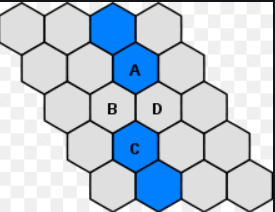
\includegraphics[scale=1]{2bridge.png}
    \caption{A two bridge A-C}
    \label{fig:2bridge}
\end{figure}

\subsection{Composants connexes et plus court chemin}

Le joueur \textit{TrustMeRushB} (présent dans le fichier \textit{projet\_jam.c} utilise une stratégie basée sur la recherche de chemin le plus court en considérant les tuiles qu'il a déjà posé. L'idée de ce joueur est de terminer la partie le plus vite possible. Pour avoir un avantage dans sa course, ce joueur essaie toujours d'avoir le premier coup. C'est pourquoi il propose un coup aléatoire en coup d'ouverture (en espérant que l'adversaire ne le décline pas) et refuse toujours le coup d'ouverture adverse.
La stratégie calcule le chemin le plus court entre les deux bouts du plateau. C'est à dire l'ensemble de tuiles à poser de taille minimale qui permettrait au joueur de gagner. Pour cela, la fonction $parcours\_largeur$ va être utilisée. Celle-ci va pour un graphe donné, un sommet de départ et un ensemble de sommets d'arrivée, retourner le chemin le plus court les reliants à l'aide d'un parcours en largeur. Dans ce parcours, quatre cas de figure peuvent se produire :

\begin{itemize}
    \item Soit le voisin v de la case étudiée u est libre. On ajoute alors v à la liste des sommets à étudier et le père de v devient u.
    \item Soit le voisin v de la case étudiée u appartient à l'adversaire ou a déjà été étudiée. On passe alors à l'étude d'un autre voisin de u.
    \item Soit le voisin v de la case étudiée u fait partie d'une composante connexe (d'un élément ou plus) de coups déjà joués. On va alors ajouter tous les voisins w des sommets de la composante connexe et leur père deviendra u. De ce fait, les composantes connexes nous permettent de "gagner des coups" pour rejoindre les deux côtés du plateau.
    \item Soit le voisin v de la case étudiée u fait partie de la liste des sommets d'arrivée. On remonte alors la liste des pères des sommets en partant de v jusqu'à arriver au sommet initial. Cette liste est ensuite retournée par la fonction.
\end{itemize}


Pour décider quelle tuile de la liste il va jouer, le joueur choisit la tuile de l'ensemble la plus proche en ligne de celle jouée précédemment par le joueur adverse. Ce comportement est fait pour que le joueur, en plus de se rapprocher de la victoire, tente de bloquer par la même occasion le joueur adverse qui voudrait également foncer vers la victoire(en faisant une ligne droite par exemple).

\newpage

\section {Tests effectués}
Afin de s'assurer de la robustesse de nos structures ainsi que de la correction de nos algorithmes, nous avons tout au long du projet élaboré plusieurs tests. Il suffit de taper la séquence des commandes suivantes:
\begin{itemize}
    \item $make$ (le rôle de cette commande sera expliqué plus tard dans la section suivante).
    \item $make$ $install$ (le rôle de cette commande sera expliqué plus tard dans la section suivante).
    \item $make$ $test$ : qui compile et exécute l'exécutable des tests $alltests$.
\end{itemize}
 L'exécutable $alltests$ est compilé avec $-lgcov$. Il exécute tous les tests présents dans le code. En particulier, il sert d'outil de mesure de la couverture des tests avec $gcov$.
 
 Les tests utilisent une structure \textit{test\_module} écrite pour ce projet. Elle permet de faciliter l'écriture des tests et leur affichage. A l'inverse des fonctions \textit{assert}, les tests du module n'arrêtent pas le programme. A la place, ils affichent le ratio des tests échoués par rapport au nombre total de tests pour ce module.
 
\section{Conclusion }
\subsection{Programme et ses options}
\subsubsection{Code principal}
Afin de démarrer une petite partie de $hex$ entre deux clients $player1$ et $player2$, nous vous prions de suivre les instructions suivantes:
\begin{itemize}
    \item $make$ compile l'ensemble du code.
    \item $make$ $install$ copie les exécutables (un exécutable nommé $server$, un exécutable $alltests$, et un nombre non spécifié de fichiers $.so$) à l'intérieur du répertoire désigné $install$.
    \item \textit{./install/server -m [M] -t [T] ./install/player1.so ./install/player2.so} démarre une partie du jeu avec un plateau du jeu de format $t$ de longueur de cote $m$ avec les deux clients. Cette syntaxe n'est pas hyper sensible à l'ordre des arguments: les variables $m$ et $t$ peuvent être définies au débit ou à la fin des arguments, sinon des valeurs par défaut seront utilisées.
\end{itemize}

\subsubsection{Code de test}
En lançant la commande $make$ $test$ dans le terminal, les codes de test sont directement compilés et exécutés. Il s'affiche alors à l'écran le nombre de tests réussis par catégorie de test, puis le nombre global de tests réussis.

\subsection{Difficultés rencontrées}

\subsubsection{Stratégies non abouties}

Nous avons essayé d'implémenter les stratégies basées sur le courant électrique de Kirchhoff et les connexions virtuelles mais n'avons pas réussi grandement en partie d'un manque de temps. Nous pensons nous être trop éparpillés et avons sous-estimé la tâche de travail que représentait ces deux stratégies. Le fichier \textit{graph\_analysis.c} contient l'ébauche faite pour implémenter les connexions virtuelles. L'échec du développement de cette stratégie est en grande partie dû à une structure beaucoup trop compliquée à maintenir.

Nous avons été pris par le temps, et en réponse à cela, nous avons décidé de nous rassembler pour développer une nouvelle stratégie délaissant donc les stratégies ayant une trop grande barrière à l'entrée pour former une équipe à temps.

Ce genre d'incident nous a appris à quel point correctement identifier et mesurer les charges de travail était important. L'importance et l'intérêt de programmer de manière incrémentale a également été soulignée. De cette manière, on peut plus facilement faire des constats sur l'avancée du projet. On peut alors ensuite les reporter aux contraintes du projet (en complexité comme en durée de développement) pour corriger les dérives.

\subsubsection{Communication et coordination}
Il a été parfois difficile d'échanger sur le projet dans les conditions de télé-travail. En particulier lorsque des explications sur des notions un peu complexes sont demandées. Les humeurs de la connexions Internet ont aussi été quelque peu problématiques lors d'explications vocales.

De ce fait, se coordonner a été un peu compliqué lorsque les communications passaient mal (voire pas du tout) surtout car nous n'avions pas de document de référence sur l'avancement du projet et l'attribution de tâches. Avoir ce genre de document peut être pratique, mais nous avons jugé qu'il était préférable de ne pas imposer de contraintes fortes sur les charges de travail et de maximiser une atmosphère de travail amicale (surtout dans cette situation).

\subsubsection{Retour sur expérience}

Le sujet de Hex a été pour nous un réel défi. En outre les nouvelles compétences demandées par rapport au premier projet S5 comme la compilation, ce projet nous a permis de fortifier notre maîtrise du C mais également notre travail d'équipe. Travailler à quatre est plus difficile à organiser qu'à deux surtout lorsqu'il nous impossible d'échanger face à face. Mais nous avons su pallier à ces problèmes et nous adapter en conséquence.

\section{Remerciements}
Nous remercions tout d'abord M. David RENAULT pour les remarques, aides,  observations mais aussi la bonne humeur qui nous ont été données soit par $SLACK$, soit par courriel, ainsi que pour l'élaboration de ce projet original. De plus, nous remercions M. Guillaume MERCIER, qui nous a accompagné tout au long du projet en nous encadrant et en répondant à toutes nos questions. Ses réflexions sur l'importance de la rigueur dans la programmation nous ont été utiles pour ce projet et nous seront probablement utiles pour le reste de notre vie de programmeur. 

\newpage
\section{Références}
\subsection{Internes}
\begin{itemize}
    \item \url{https://www.labri.fr/perso/renault/working/teaching/projets/}
    \item \url{https://www.labri.fr/perso/renault/working/teaching/projets/2019-20-S6-C-Hex.php}
\end{itemize}
\subsection{Externes}
\begin{itemize}
    \item \url{https://www.youtube.com/watch?v=2MNalT1g3m8}
    \item \url{http://www.lutanho.net/play/hex.html}
    \item \url{https://www.gnu.org/software/gsl/doc/html/index.html}
    \item \url{https://pdfs.semanticscholar.org/2a99/60b28c01526d7b04e4dda7d82e2c59c9bcf1.pdf}
    \item \url{https://www.aaai.org/Papers/AAAI/2000/AAAI00-029.pdf}
    \item \url{https://www.overleaf.com/}
    \item \url{https://fr.wikipedia.org/wiki/Algorithme_minimax}
\end{itemize}

\newpage
\section{Annexes}
\begin{figure}[ht]
    \centering
\begin{lstlisting}
struct graph_t* hexa_graph__empty(int m){
  int vertices = (m+1) * (m+1);
  struct graph_t* g = graph__empty (vertices);
  int line_length = m+1;
  for (int i = 0; i < vertices; i++){
    int index = i%line_length;
    // Adds right links
    if (index+1 < line_length)
      gsl_spmatrix_set(g -> t, i, i+1, 1);
    // Adds left links
    if (index-1 >= 0)
      gsl_spmatrix_set(g -> t, i, i-1, 1);
    // Adds down links
    if (i/line_length < line_length-1 && index > 0)
      gsl_spmatrix_set(g -> t, i, i+line_length - 1, 1);  
    if (i+line_length < vertices && i/line_length < line_length-1)
      gsl_spmatrix_set(g -> t, i, i+line_length, 1);
    // Adds up links
    if (i/m > 0 && index < line_length-1)
      gsl_spmatrix_set(g -> t, i, i-line_length + 1, 1);  
    if (i-line_length >= 0 && i/line_length > 0)
      gsl_spmatrix_set(g -> t, i, i-line_length, 1);
    // Ownership of initial boxes
    for (int i = 0; i < line_length-1; i++){
      gsl_spmatrix_set(g -> o, 0, i, 1);
      gsl_spmatrix_set(g -> o, 0, vertices-1-i, 1);
      gsl_spmatrix_set(g -> o, 1, (i+1)*line_length, 1);  
      gsl_spmatrix_set(g -> o, 1, vertices-1-(i+1)*line_length, 1); 
    }
  }
  return g;
}

\end{lstlisting}
    \caption{Function representing an empty hexagonal grid}
    \label{fig:graph_hex}
\end{figure}

\begin{figure}[ht]
    \centering
\begin{lstlisting}
struct player{
  char const* (* get_player_name)(); // sur toute fonction qui génère le nom du joueur
  struct move_t (* propose_opening)(); // sur toute fonction qui propose le premier coup
  int (*accept_opening)(const struct move_t opening);// sur toute fonction qui accepte ou pas le premier coup
  void (*initialize_graph)(struct graph_t* graph);// sur toute fonction qui initialise le graphe du joueur
  void (*initialize_color)(enum color_t id);// sur toute fonction qui initialise la couleur du joueur
  struct move_t (*play)(struct move_t previous_move);// sur toute fonction qui propose des coups en se basant sur le dernier coup de l'adversaire
  void (*finalize)();// sur toute fonction qui libère tout ce qui est alloué 
};
\end{lstlisting}
    \caption{$struct$ $player$}
    \label{fig:player}
\end{figure}

\begin{figure}[ht]
\begin{lstlisting}
struct player make_player(void* handle){
  struct player p;
  p.get_player_name=dlsym(handle, "get_player_name");
  p.propose_opening=dlsym(handle,"propose_opening");
  p.accept_opening=dlsym(handle, "accept_opening");
  p.initialize_graph=dlsym(handle, "initialize_graph");
  p.initialize_color=dlsym(handle, "initialize_color");
  p.play=dlsym(handle, "play");
  p.finalize=dlsym(handle, "finalize");
  p.color=NO_COLOR;
  return p;
}
\end{lstlisting}
    \caption{Making of a $player$}
    \label{fig:making_of_player}
\end{figure}

\begin{figure}[ht]
\begin{lstlisting}
void graph__free (struct graph_t* g){
  assert (g != NULL);
  gsl_spmatrix_free(g -> o);
  gsl_spmatrix_free(g -> t);
  free(g);
}
\end{lstlisting}
    \caption{$graph\_free$}
    \label{fig:free}
\end{figure}

\begin{figure}[ht]
\begin{lstlisting}
size_t minimax(size_t position, size_t depth, int alpha, int beta, int maximizing){
     if (depth == 0 ){ // || is_winning()
            return position;
     }

     if (maximizing){
        int besteval = - 1000;
        size_t bestpos = position;
        for (int i=0; i < (m+1)*(m+1); i++){
            if (!is_owned(i)){
                size_t pos = minimax(i, depth - 1, alpha, beta, FALSE);
                int old_besteval = besteval;
                besteval = max(besteval, evaluation(pos));
                if (besteval != old_besteval)
                    bestpos = pos;
                alpha = max(alpha, pos);
                if (beta <= alpha)
                    break;   
            }
        }
        return bestpos;
     }
     else{
        int leasteval = 1000;
        size_t leastpos = position;
        for (int i = last_position; i < (m+1)*(m+1); i++){
            if (!is_owned(i)){
                int pos = minimax(i, depth - 1, alpha, beta, TRUE);
                int old_leasteval = leasteval;
                leasteval = min(leasteval, evaluation(pos)); 
                if (leasteval != old_leasteval)
                    leastpos = pos; 
                beta = min(beta, pos);
                if (beta <= alpha)
                    break;  
            }
        }
        return leastpos;
     }
 }
\end{lstlisting}
    \caption{Variante du $MinMax$}
    \label{fig:Minmax}
\end{figure}


\end{document}